\documentclass[12pt]{article}
\usepackage{lineno}
%\usepackage{ametsoc}
\usepackage{natbib}
\usepackage{a4wide}
\usepackage{amsfonts}
\usepackage{amssymb}

\usepackage{color}
\usepackage[pdftex]{graphicx}
\usepackage[pdftex,colorlinks, citecolor=black,linkcolor=black,urlcolor=black]{hyperref}
\definecolor{darkgreen}{rgb}{0.1,0.4,0.1}
\definecolor{darkblue}{rgb}{0.1,0.1,0.3}



\newif\ifdetail
\global\detailfalse
%\global\detailtrue

\def\bem#1{\colorbox{green}{\em #1}}

\newcommand{\beq}  { \begin{eqnarray} }
\newcommand{\eeq}  { \end{eqnarray}}
\newcommand{\beeq}  { \begin{eqnarray*} }
\newcommand{\eeeq}  { \end{eqnarray*}}
\newcommand{\eq }  [1]{Eq.~(\ref{#1})}  % Eq. (#1)
\newcommand{\eqs }  [1]{Eqs.~(\ref{#1})}
\newcommand{\sect}  [1]{Sec.~(\ref{#1})}  % Eq. (#1)
\newcommand{\fig}  [1]{Fig.~\ref{#1}}   % Fig. #1
\renewcommand{\v}[1]{{\mbox{\boldmath$ #1 $}}}  % Vektor durch Fettdruck
\newcommand{\m}    [1]{{\bf  #1 }}              % Matrix in sans serif
\newcommand{\gz}[1] {{{d #1} \over {dz}}}
\newcommand{\pt}[1]{{\partial_t #1}}
\newcommand{\ptt}[1]{{{\partial^2 #1} \over {\partial t^2}}}
\newcommand{\pttx}[1]{{{\partial^3 #1} \over {\partial t^2 \partial x}}}
\newcommand{\ptty}[1]{{{\partial^3 #1} \over {\partial t^2 \partial y}}}
\newcommand{\pttt}[1]{{{\partial^3 #1} \over {\partial t^3}}}
\newcommand{\ptx}[1]{{{\partial^2 #1} \over {\partial t \partial x}}}
\newcommand{\pty}[1]{{{\partial^2 #1} \over {\partial t \partial y}}}
\newcommand{\pz}[1]{{\partial_z #1}}
\newcommand{\pzz}[1]{{\partial_{zz} #1}}
\newcommand{\px}[1]{{\partial_x #1}}
\newcommand{\py}[1]{{\partial_y #1}}
\newcommand{\pxi}[1]{{\partial_i #1}}
\newcommand{\pxj}[1]{{\partial_j #1}}
\newcommand{\pxk}[1]{{\partial_k #1}}
\newcommand{\pb}[1]{{{\partial #1} \over {\partial b}}}
%\newcommand{\pxy}[1]{{{\partial^2 #1} \over {\partial x \partial y}}}
\newcommand{\pxy}[1]{\partial_{xy} #1}
\newcommand{\pyy}[1]{\partial_{yy} #1}
\newcommand{\pxx}[1]{\partial_{xx} #1}
\newcommand{\kx}{{\bf k} \times}
\newcommand{\dt}[1]{{{d #1} \over {d t}}}
\newcommand{\Dt}[1]{{{D #1} \over {D t}}}
\newcommand{\Div}[1]{ \nabla \cdot #1 }
\renewcommand{\div}[1]{ \nabla_{yz} \cdot #1 }
\newcommand{\Bar}[1]{ \overline{ #1} }
\newcommand{\rvec} [1]{
    \raisebox{-1.5ex}{$\stackrel{\textstyle #1}{\neg}$} }% rotierter Vektor
\newcommand{\nablq}   {\rvec\nabla}                    % rotated nabla operator
\newcommand{\Vec}[1]{\left(\begin{array}{c} #1 \end{array}\right) }
%\renewcommand{\mho}{\mathcal{W}}
\newcommand{\pn}[1]{{{\partial #1} \over {\partial n}}}
\newcommand{\pnn}[1]{{{\partial #1} \over {\partial m}}}
\newcommand{\ps}[1]{{{\partial #1} \over {\partial s}}}
\newcommand{\p}{{\partial}}
\newcommand{\vn}{{\v \nabla}}
\newcommand{\lk}{\left(}
\newcommand{\rk}{\right)}

\newcommand{\tl}{\tilde}


\newcommand{\E}{\mathcal{E}}
\newcommand{\A}{\mathcal{A}}

\newcommand{\ep}{\epsilon}

\begin{document}

\section*{The Saturn model}


Consider the non-linear barotropic or reduced gravity model 
\beq \label{eq1}
  \pt{  \v u } +  f \rvec{ \v u} +   \vn   h =   -  \v u \cdot \vn  \v u ~~,~~
    \pt{ h}  + { c}^2  \vn \cdot  \v u    =   - \vn \cdot  h   \v u 
     \eeq
   with the Coriolis parameter $f$, the gravity wave speed $c^2$, and 
 the layer velocity $\v u$.  The layer thickness perturbation $\eta$ was re-scaled to $h = g \eta$
 with  reduced gravity $g$ such that $c^2 = g \bar \eta$, with the mean thickness $\bar \eta$.
   The vector $\rvec{\v u}$ denotes  anticlockwise rotation of the vector
$\v u$ by $\pi/2$, i.e. $\rvec{ \v u} =(-v, u)$ for $\v u=(u,v)$.
   
\subsection*{Scaling} 
   
 Using the beta plane $ f(y) =  f(0) +  f' y $, the scaling $h \sim   f U L$ from geostrophy, $x,y \sim L$, and the wave scaling
$t \sim  1/ f$, a   scaled version of \eq{eq1}  becomes
\beq \label{eq2}
\pt{\v u }    +  (\tl f + \beta y )  \rvec{\v u}  +   \vn h =  - Ro \,   \v u \cdot \vn \v u
 ~~,~~
 \pt{h}  + \tl c^2 \vn \cdot \v u    =   - Ro  \, \vn \cdot h \v u 
      \eeq
with the Rossby number $Ro = U/(  f L)$ and $\tl c=L_r/L= Ro /F$ 
where  $L_r = c/  f$ denotes the Rossby radius, with the Froude number $F=U/  c $,
 and $\beta = L/a\ll 1$, where $a$ denotes
the Earth radius. $\tl f=1$ is kept for reference.
For $Ro=1$  and $f=\tl f$, $\beta= f'$, $c=\tl c$  this becomes the dimensional version again
and thus we drop the tilde for $f$ and $c$ from now.



\subsection*{Total, kinetic, and potential energy and potential voticity}


Using the relation  $\vn \v u^2/2 + \rvec{\v u} \rvec{\vn} \cdot \v u = \v u \cdot \vn \v u$, the system \eq{eq2} 
 can be written as 
 \beq
  \pt{} \v u +q \rvec{\v U} + \vn (h + Ro \,  K) =0
  ~~,~~ \pt h + \vn \cdot\v U  = 0 
 \eeq
 with total thickness $H= c^2+Ro \,  h$, volume transport $\v U = H \v u$, kinetic energy $K= \v u^2/2 $
  and potential vorticity $q=(f + Ro \,  \rvec{\vn} \cdot \v u)/H$.
Kinetic energy $K$  is given by
\beq
\pt{ K }     + \v u \cdot   \vn h  = -  Ro \, \v u \cdot \vn K
\eeq
the term $\v u \cdot    \vn h$ is the exchange with potential energy.
Total energy $T$ is given by 
\beq 
T=Ro^2 \, H K + H^2/2
\eeq 
 obtained by adding $Ro^2 H$ times 
the kinetic energy equation and $\epsilon H$ times the thickness equation which yields
  \beq
   \pt T + Ro \,   \vn \cdot (H+ Ro^2 K) \v U    = 0
  \eeq
  Total energy is conserved since it holds that
  \beq
  \int dA \pt{}T =
 Ro \,  \int dA  \lk Ro \,     \v U \cdot \pt{} \v u+  (H    +Ro^2  K )\pt h \rk = 0
  \eeq
  


\subsection*{Linear discrete equations} 


\begin{figure}
\centerline{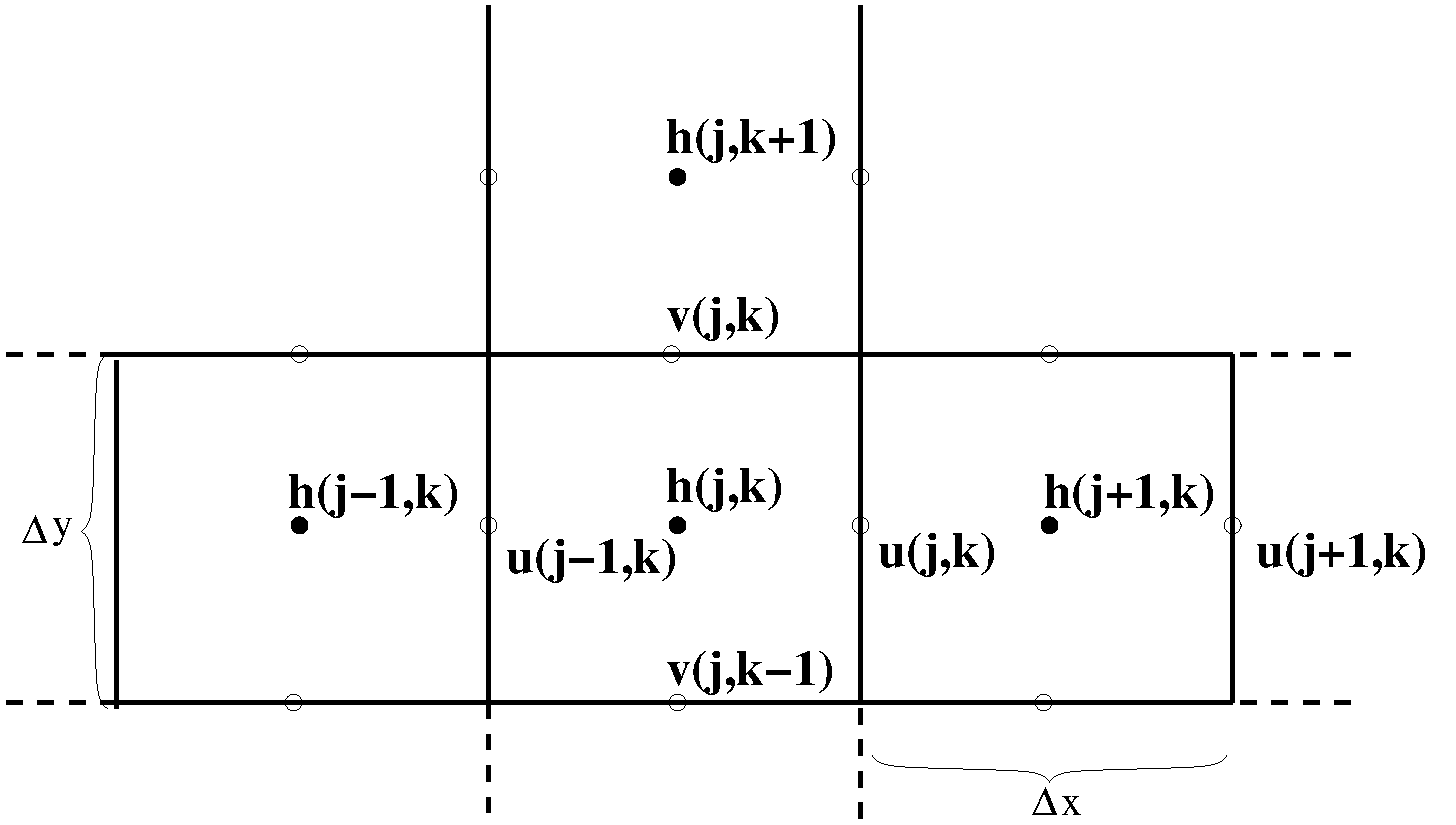
\includegraphics[width=0.8\textwidth]{cgrid} }
\caption{The staggered grid arrangement.}
\label{fig1}
\end{figure} 

Omitting the non-linear terms by setting  $Ro=0$ for the moment, 
rewrite \eq{eq2}  as
\beq
  \pt{�u} = fv  - \px h    ~~,~~ \pt{�v} = -fu  - \py h   ~~,~~ \pt h = -c^2  \lk   \px u  + \py v \rk 
   \eeq
For discretisation we use the C-grid arrangement shown in \fig{fig1} which yields
\beq
  \dt{�u_{j,k}}  =  f \Bar{\Bar{v_{j,k}}^{j+}}^{k-}    - \delta_x^+ h_{j,k} 
   ~,~
    \dt{�v_{j,k}}  = -  f \Bar{\Bar{u_{j,k}}^{j-}}^{k+}    - \delta_y^+ h_{j,k} 
      ~,~
 \dt{ h_{j,k}}  = - c^2 \lk \delta_x^- u_{j,k}  +  \delta_y^- v_{j,k}  \rk
 \eeq
 with the finite differencing operators
\beq
 \delta^+_x h_{j,k} = (h_{j+1,k} - h_{j,k})/\Delta_x
  ~~,~~
 \delta^-_x h_{j,k} = (h_{j,k} - h_{j-1,k})/\Delta_x
 \\
 \delta^+_y h_{j,k} = (h_{j,k+1} - h_{j,k})/\Delta_y
  ~~,~~
 \delta^-_y h_{j,k} = (h_{j,k} - h_{j,k-1})/\Delta_y
 \eeq
and 
with the finite averaging operators
\beq
 \Bar{h_{j,k}}^{j+} = (h_{j,k} +  h_{j+1,k} )/2 ~~,~~ 
 \Bar{h_{j,k}}^{j-} =  (h_{j,k} +  h_{j-1,k} ) /2
  \\
\Bar{h_{j,k}}^{k+} =  (h_{j,k} +  h_{j,k+1} )/2~~,~~ 
  \Bar{h_{j,k}}^{k-} = (h_{j,k} +  h_{j,k-1} ) /2
 \eeq
 
\subsection*{Non-linear discrete equations} 

For the discrete non-linear system of \eq{eq2}, we use the momentum equation in the form 
\beq
   \p_t \v u  + q  \rvec{\v U}  = -    \vn ( h + Ro \, K)
   ~~,~~   \p_t{h}   +  \vn \cdot  \v U    = 0 
   \eeq
 and discretise it using  the energy conserving scheme by Sadourny (1975).
The volume transport $\v U=(U,V) = H \v u $ with total thickness $H= c^2 + Ro \, h$ 
is defined at $u_{j,k}$ and $v_{j,k}$ points
 \beq
   U_{j,k} = u_{j,k} \Bar{ H}^{j+} ~~,~~V = v_{j,k} \Bar{H}^{k+}~~\to~~\dt{ h_{j,k}}  =-  \delta_x^{-} U_{j,k} -  \delta_y^{-} V_{j,k}
 \eeq
Potential vorticity $q$ is defined at grid corners as 
  \beq
    q_{j,k}=  \lk f+ \delta_x^{+} v_{j,k}   - \delta_y^+ u_{j,k}  \rk / \Bar{  \Bar{H}^{j+}  }^{k+} 
  \eeq
The gradient force in momentum equation is given by
\beq
p_{j,k}= (h + Ro \, K)_{j,k} = h_{j,k} + Ro \,  ( \Bar{u_{j,k}^2}^{j-} + \Bar{v_{j,k}^2}^{k-} )/2 
\eeq
and the 
momentum equation is then discretized as
\beq
 \dt{ u_{j,k}}  =   \Bar{ q_{j,k} \Bar{V_{j,k}}^{j+}  }^{k-}  - \delta_x^+ p_{j,k}
 ~~,~~\dt{ v_{j,k}  } =  - \Bar{ q_{j,k} \Bar{U_{j,k}}^{k+}  }^{j-}  - \delta_y^+ p_{j,k}
\eeq
It can be shown for the discrete equations that total energy $T$ is indeed conserved by this scheme.
However, it is much easier to check this in the code.



\end{document}